\section{Diseño del software}

El software articula datos, entrenamiento, almacenamiento, despliegue e interfaz web. La base de datos de entrenamiento se construye vinculando imágenes heliográficas con reportes observacionales, de modo que las etiquetas Zurich--McIntosh y los metadatos temporales puedan usarse para entrenar y auditar modelos de detección y clasificación \citep{noaaSRS,scherrer2012hmi,bobra2014sharp,robUSET2026}.

\subsection{Obtención y preparación de datos}

Los datos se obtuvieron acoplando imágenes fotosféricas SDO/HMI de disco completo con reportes diarios NOAA SRD/SRS para el período 2010--2025. DB1 conserva el disco completo con cajas de grupos solares obtenidas a partir de proyecciones heliográficas y filtros como el \textit{black-hat}; DB2 contiene recortes normalizados de $224\times224$; y DB2.1 refina esos recortes mediante detecciones YOLO26n y realce morfológico para mejorar la correspondencia entre imagen, posición y etiqueta \citep{scherrer2012hmi,noaaSRS,cesarHeliographic,robUSET2026}.

\begin{table}[H]
\centering
\caption{Resumen de bases de datos utilizadas para entrenamiento y refinamiento. \textbf{Fuente:} Elaboración propia a partir del flujo de construcción de datos.}
\label{tab:resumen-bases-datos}
%\scriptsize
\begin{tabular}{lp{0.25\linewidth}cp{0.30\linewidth}}
\toprule
\textbf{Base} & \textbf{Observación} & \textbf{Registros} & \textbf{Uso principal} \\
\midrule
DB1 & Disco completo & $\sim$4700 & Entrenamiento de YOLO26n \\
DB2 & Grupo solar & $\sim$15000 & Etapa intermedia \\
DB2.1 & Grupo solar refinado (Yolo26n+PCA) & $\sim$14300 & Entrenamiento de ConvNeXtV2a \\
\bottomrule
\end{tabular}
\end{table}

\subsection{Detección de grupos solares}

El detector YOLO26n localiza grupos solares y produce recortes que reducen el dominio visual para la clasificación; las curvas de pérdida, precisión, \textit{recall} y mAP permiten verificar la convergencia del detector y su utilidad para construir recortes consistentes \citep{ultralyticsYOLO26,robUSET2026,noaaSRS}.

\begin{figure}[H]
    \centering
    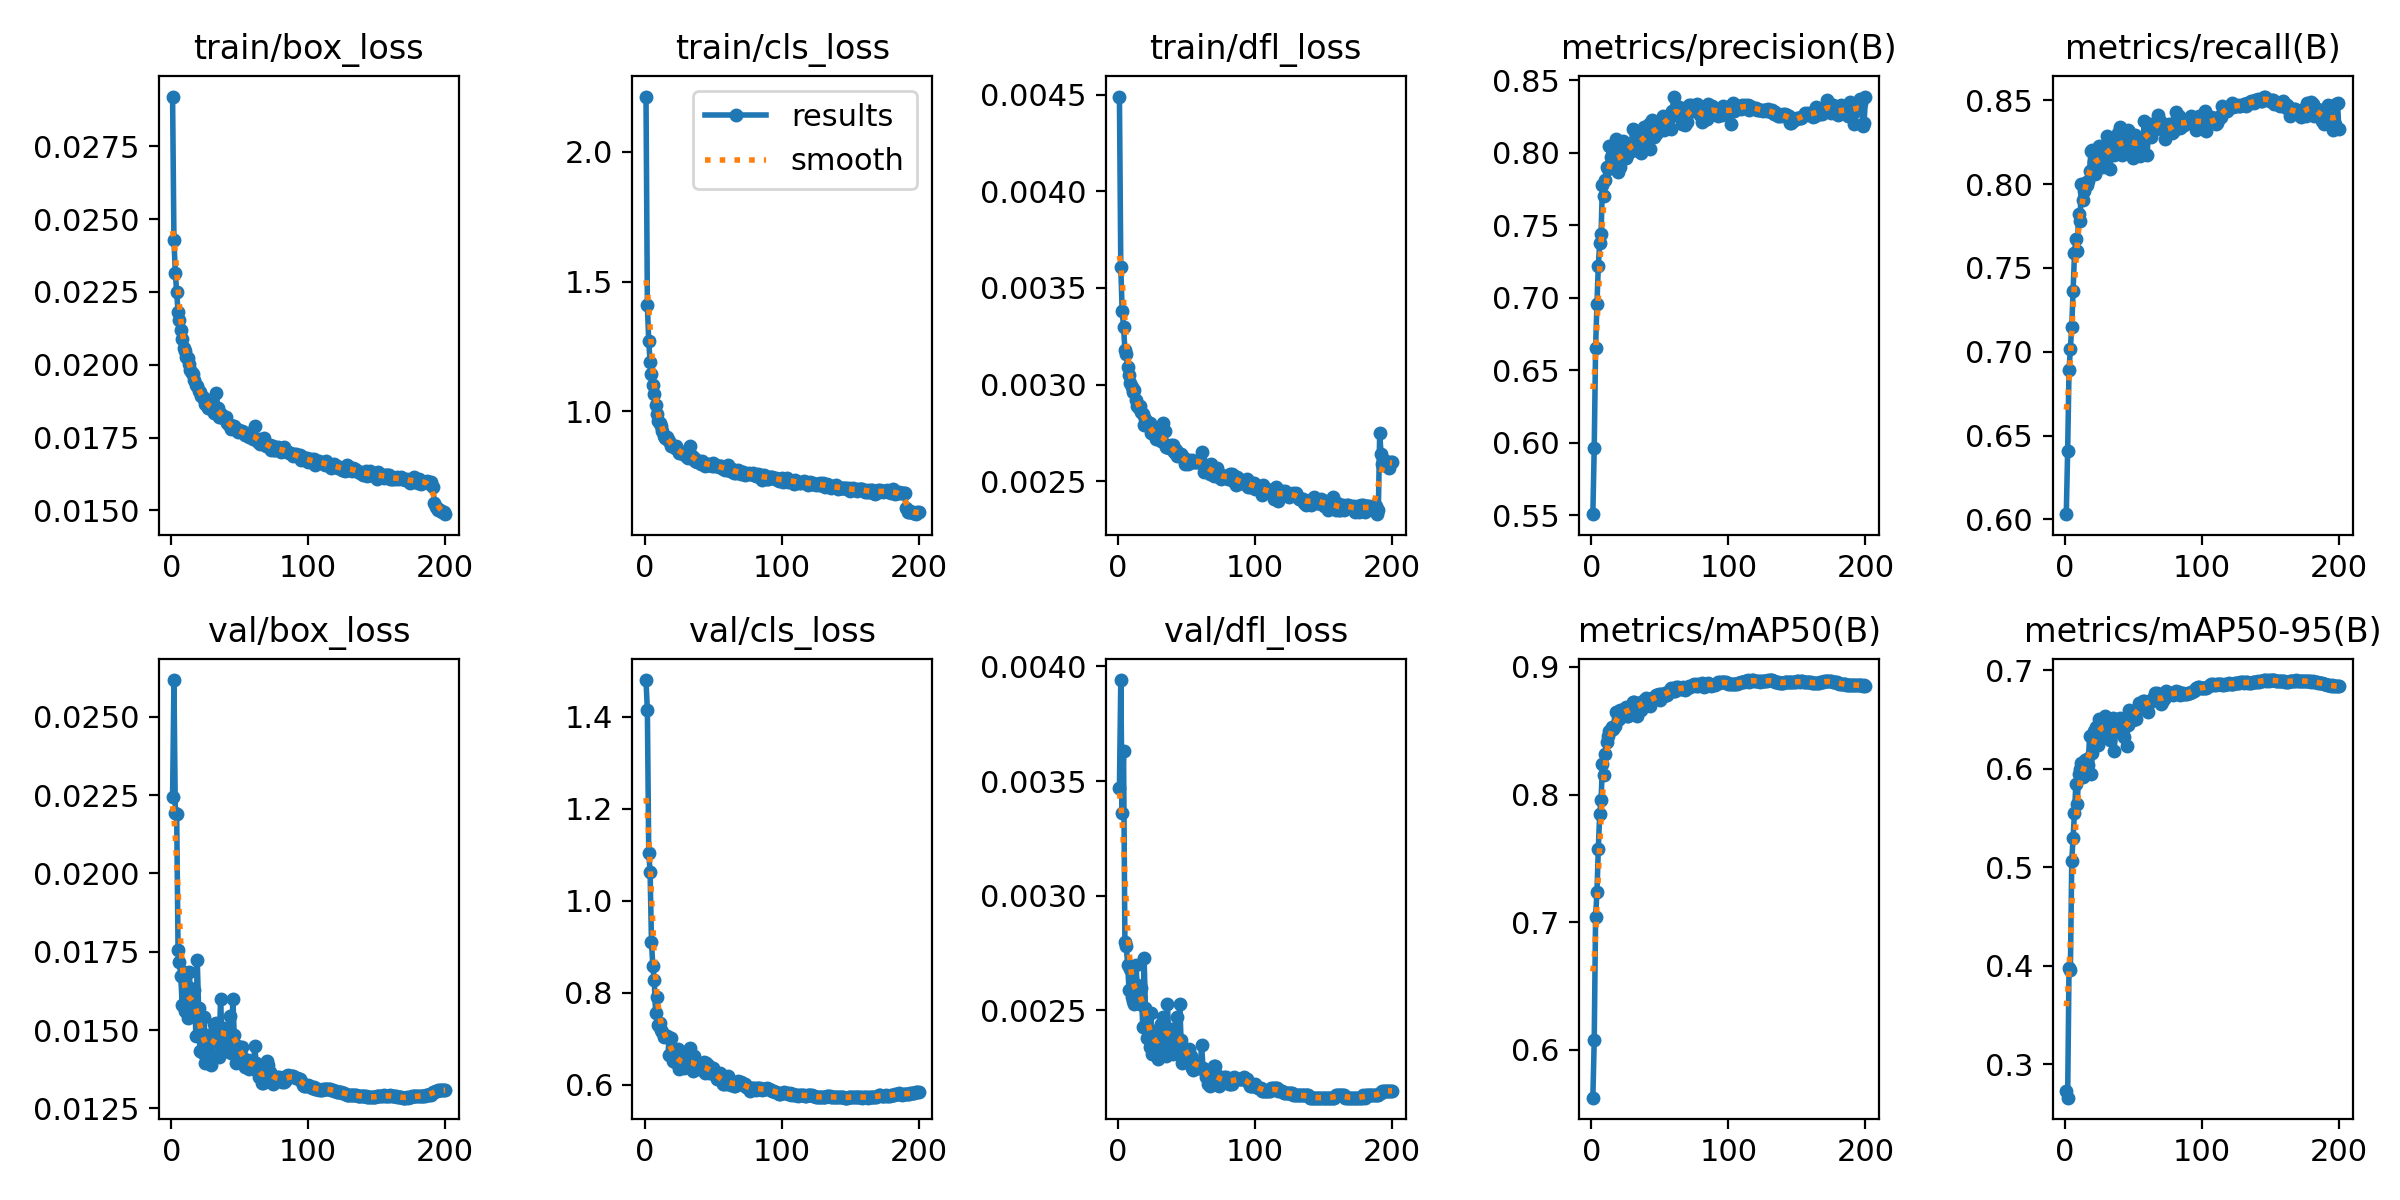
\includegraphics[width=0.92\linewidth]{figures/ml/yolo_results.png}
    \caption{Métricas de entrenamiento del detector YOLO26n sobre DB1, incluyendo pérdidas de entrenamiento/validación, precisión, \textit{recall} y mAP. \textbf{Fuente:} Elaboración propia.}
    \label{fig:resumen-yolo-training}
\end{figure}

\subsection{Clasificación jerárquica Zurich--McIntosh}

Luego, ConvNeXtV2 Atto opera como extractor compacto de características para los recortes normalizados de regiones activas. Esta división separa localización y descripción morfológica, reduce la complejidad frente a una clase plana $ZPC$ y preserva la interpretación astronómica de cada salida \citep{woo2023convnextv2,mcintosh1990classification,zhou2023mcintosh}.

\begin{figure*}[t]
    \centering
    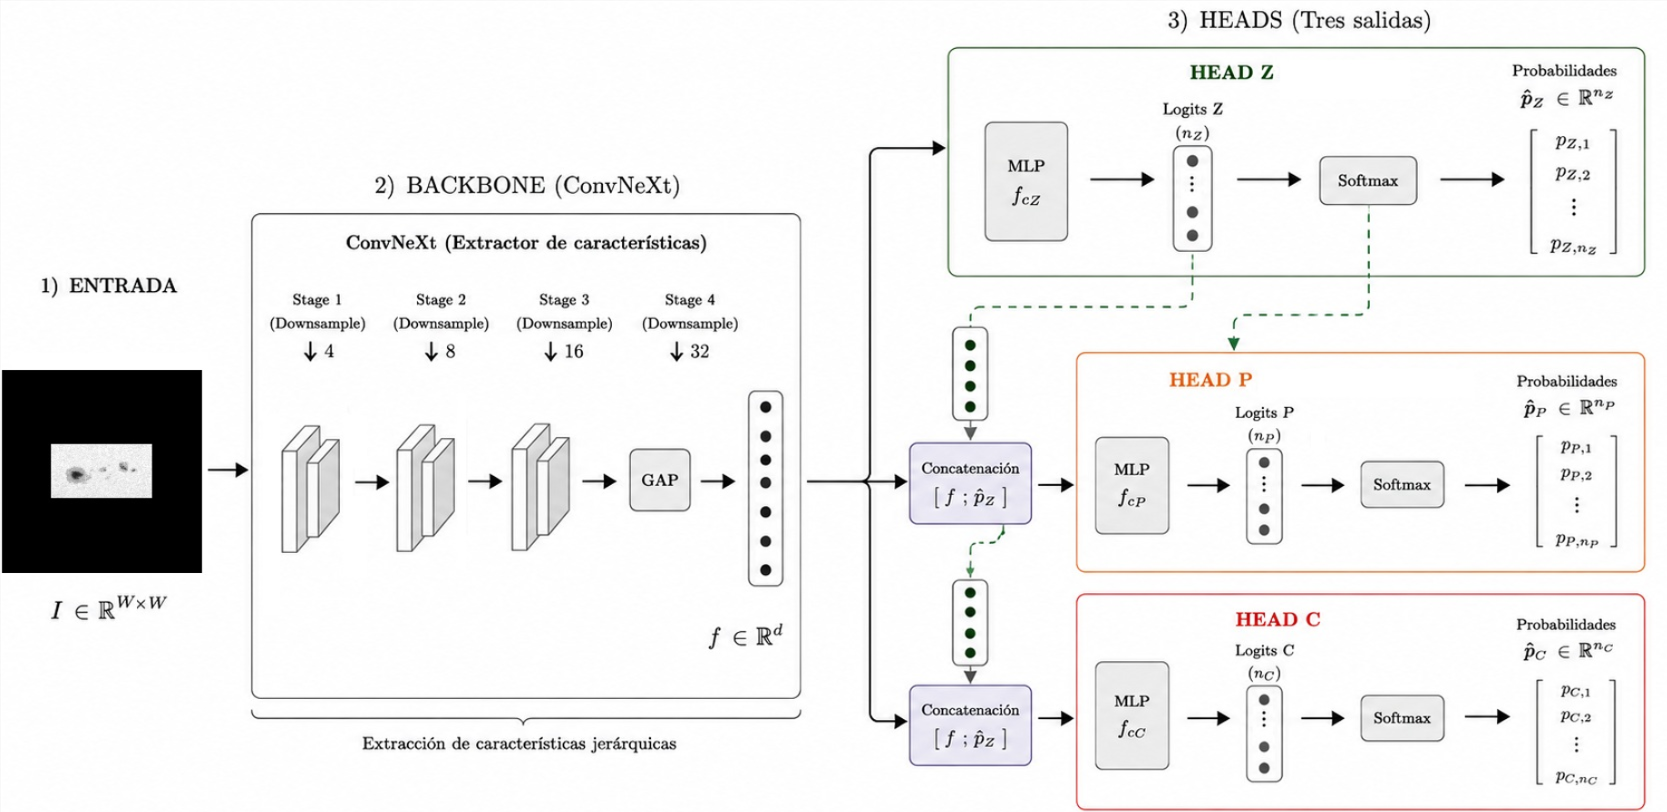
\includegraphics[width=0.98\textwidth]{figures/ml/convnext_arch.png}
    \caption{Arquitectura de clasificación jerárquica basada en ConvNeXtV2 para componentes Zurich--McIntosh. El recorte solar se transforma mediante el extractor ConvNeXtV2; luego, el agrupamiento promedio global produce el vector latente $\mathbf{f}$, a partir del cual se calcula primero la distribución $\hat{\mathbf{p}}_Z$. Las salidas $P$ y $C$ usan la concatenación $[\mathbf{f};\hat{\mathbf{p}}_Z]$ para incorporar dependencia jerárquica antes de la recomendación final. \textbf{Fuente:} Elaboración propia con base en ConvNeXtV2.}
    \label{fig:resumen-convnext}
\end{figure*}

La Figura~\ref{fig:resumen-convnext} resume el flujo jerárquico del clasificador. Para un recorte $x\in\mathbb{R}^{224\times224}$, el backbone ConvNeXtV2 produce mapas de características que se resumen mediante agrupamiento promedio global en un vector
\begin{equation}
\mathbf{f}=\operatorname{GAP}(\operatorname{ConvNeXtV2}(x)), \qquad \mathbf{f}\in\mathbb{R}^{d}.
\end{equation}
La primera salida estima la distribución del carácter Zurich,
\begin{equation}
\hat{\mathbf{p}}_Z=\operatorname{softmax}(g_Z(\mathbf{f})), \qquad \hat{\mathbf{p}}_Z\in\mathbb{R}^{n_Z}.
\end{equation}
Luego, las salidas penumbral y de compactación incorporan la dependencia con $Z$ usando la concatenación del vector visual y la distribución Zurich:
\begin{equation}
\hat{\mathbf{p}}_P=\operatorname{softmax}(g_P([\mathbf{f};\hat{\mathbf{p}}_Z])), \qquad
\hat{\mathbf{p}}_C=\operatorname{softmax}(g_C([\mathbf{f};\hat{\mathbf{p}}_Z])).
\end{equation}
Por tanto, el clasificador se expresa como
\begin{equation}
f_\theta(x)=\left(\hat{\mathbf{p}}_Z,\hat{\mathbf{p}}_P,\hat{\mathbf{p}}_C\right),
\end{equation}
donde cada término es una distribución probabilística sobre una componente de la taxonomía. Esta formulación conserva la estructura semántica Zurich--McIntosh y facilita la exportación del modelo a ONNX como un sistema multisalida \citep{woo2023convnextv2,mcintosh1990classification}.

\subsection{Posprocesamiento probabilístico}

El posprocesamiento convierte las tres salidas del clasificador en una recomendación probabilística restringida al espacio válido de clases Zurich--McIntosh. Para una imagen $x$, la probabilidad conjunta ideal se expresa como
\begin{equation}
P(Z,P,C\mid x)=P(Z\mid x)P(P\mid Z,x)P(C\mid Z,P,x).
\end{equation}
Como implementación operativa se usa una base factorizada,
\begin{equation}
P_{\mathrm{base}}(Z,P,C\mid x)=P(Z\mid x)P(P\mid x)P(C\mid x),
\end{equation}
y se aplica una máscara binaria $M_{ZPC}$ para anular combinaciones no admisibles. La distribución recomendada queda normalizada como
\begin{equation}
P_{\mathrm{rec}}(Z,P,C\mid x)=
\frac{P_{\mathrm{base}}(Z,P,C\mid x)M_{ZPC}}
{\sum_{z,p,c}P_{\mathrm{base}}(z,p,c\mid x)M_{zpc}}.
\end{equation}
La clase final se obtiene con $(Z^\ast,P^\ast,C^\ast)=\arg\max_{Z,P,C}P_{\mathrm{rec}}(Z,P,C\mid x)$, manteniendo interpretabilidad y consistencia taxonómica \citep{mcintosh1990classification,sayez2023sunscc}.

\subsection{Modelos predictivos}

Para los modelos predictivos, el número de manchas solares suavizado se estima con PVL--Kalman. La etapa de actualización queda dada por
\begin{equation}
K_k=P_k^{-}(P_k^{-}+R_k)^{-1}, \qquad
\widehat{s}_k=\widehat{s}_k^{-}+K_k(z_k-\widehat{s}_k^{-}),
\end{equation}
donde $z_k$ es la observación mensual y $\widehat{s}_k$ la estimación corregida. Este bloque resume la amplitud temporal del ciclo solar mediante una serie escalar \citep{kalman1960newapproach,podladchikova2012kalman}.

El modelo DMD complementa esa salida escalar con una reconstrucción de la distribución latitudinal de actividad. Cada observación mensual se transforma en un vector de conteos latitudinales. Sea $N_{\mathrm{spots}}(t)$ el número total de manchas en el instante $t$ y $\theta_i(t)$ la latitud heliográfica de la $i$-ésima mancha; el dominio se restringe a
\begin{equation}
\theta\in[-50^{\circ},50^{\circ}], \qquad \Delta\theta=4^{\circ}, \qquad M=25.
\end{equation}
El $j$-ésimo contenedor se define como $\mathcal{B}_j=[\theta_j,\theta_{j+1})$ y su conteo como
\begin{equation}
V_j(t)=\sum_{i=1}^{N_{\mathrm{spots}}(t)}\Psi_{j,i}(t), \qquad
\Psi_{j,i}(t)=
\begin{cases}
1, & \theta_i(t)\in\mathcal{B}_j,\\
0, & \theta_i(t)\notin\mathcal{B}_j,
\end{cases}
\end{equation}
de modo que $\Psi_{j,i}(t)$ actúa como función indicadora de pertenencia de la mancha $i$ al contenedor latitudinal $j$.
Con ello, el estado latitudinal mensual queda dado por
\begin{equation}
\mathbf{x}_t=\begin{bmatrix}V_1(t)&V_2(t)&\cdots&V_M(t)\end{bmatrix}^{T}\in\mathbb{R}^{M},
\end{equation}
y la secuencia histórica se organiza como matriz de instantáneas:
\begin{equation}
\mathbf{X}=\begin{bmatrix}\mathbf{x}_1&\mathbf{x}_2&\cdots&\mathbf{x}_N\end{bmatrix}\in\mathbb{R}^{M\times N}.
\end{equation}

La Descomposición en Modos Dinámicos aproxima la evolución mediante un operador lineal efectivo $\mathbf{A}$, de modo que
\begin{equation}
\mathbf{x}_{k+1}\approx\mathbf{A}\mathbf{x}_{k}.
\end{equation}
A partir de $\mathbf{X}$ se construyen matrices desplazadas de estados consecutivos:
\begin{equation}
\mathbf{X}_1=\begin{bmatrix}\mathbf{x}_1&\cdots&\mathbf{x}_{N-1}\end{bmatrix},\quad
\mathbf{X}_2=\begin{bmatrix}\mathbf{x}_2&\cdots&\mathbf{x}_{N}\end{bmatrix}.
\end{equation}
El operador se estima con una SVD truncada de rango $r=10$,
\begin{equation}
\mathbf{X}_1\approx\mathbf{U}_r\boldsymbol{\Sigma}_r\mathbf{V}_r^{H},
\end{equation}
y se reconstruye como
\begin{equation}
\mathbf{A}\approx\mathbf{X}_2\mathbf{V}_r\boldsymbol{\Sigma}_r^{-1}\mathbf{U}_r^{H}.
\end{equation}
La proyección futura se calcula iterativamente mediante
\begin{equation}
\widehat{\mathbf{x}}_{k+1}=\mathbf{A}\widehat{\mathbf{x}}_k, \qquad k>N.
\end{equation}
Finalmente, el índice global derivado de DMD se obtiene integrando la distribución latitudinal predicha:
\begin{equation}
\widehat{\mathbf{x}}_t=\begin{bmatrix}\widehat{V}_1(t)&\widehat{V}_2(t)&\cdots&\widehat{V}_M(t)\end{bmatrix}^{T},
\end{equation}
\begin{equation}
\mathrm{SSN}_{\mathrm{DMD}}(t)=\kappa\sum_{j=1}^{M}\widehat{V}_j(t), \qquad
\kappa=\frac{\sum_{t=1}^{N}\mathrm{SSN}_{\mathrm{obs}}(t)}{\sum_{t=1}^{N}\sum_{j=1}^{M}\widehat{V}_j(t)}.
\end{equation}
Estas ecuaciones permiten pasar de una representación latitudinal física a una magnitud comparable con el SSN histórico, sin perder la lectura espacio-temporal del diagrama de Spörer \citep{schmid2010dmd,kutz2016dmd,hathaway2015solarcycle}.

\subsection{Plataforma web e inferencia portable}

La plataforma web se implementa con una lógica de consulta, visualización e inferencia portable. La conversión de modelos a ONNX permite ejecutar inferencia en entornos locales o de navegador, disminuyendo dependencia de un servidor central y facilitando uso en condiciones de conectividad limitada \citep{woo2023convnextv2,ultralyticsYOLO26,camporeale2019ml}.